% ------------------------------------------------------------------------
% ------------------------------------------------------------------------
% Desenho da aplicação LIXT, para a disciplina PI1A5
% Equipe TGT
% 1° semestre de 2021
% ------------------------------------------------------------------------
% ------------------------------------------------------------------------

\documentclass[
	% -- opções da classe memoir --
	12pt,
	openright,
	oneside,
	a4paper,
	% -- opções do pacote babel --
	english,
	brazil
  ]{abntex2}

\usepackage{lmodern}
\usepackage[T1]{fontenc}
\usepackage[utf8]{inputenc}
\usepackage{lastpage}
\usepackage{indentfirst}
\usepackage{color}
\usepackage{graphicx}
\usepackage{microtype}

\usepackage[brazilian,hyperpageref]{backref}
\usepackage[alf]{abntex2cite}

\renewcommand{\backrefpagesname}{Citado na(s) página(s):~}
\renewcommand{\backref}{}
\renewcommand*{\backrefalt}[4]{
	\ifcase #1 %
		Nenhuma citação no texto.%
	\or
		Citado na página #2.%
	\else
		Citado #1 vezes nas páginas #2.%
	\fi}%

% ---
\titulo{
  \ABNTEXchapterfont\bfseries\LARGE Lixt\\
  \ABNTEXchapterfont\mdseries\Large Desesenho da aplicação
}
\autor{Alkindar José Ferraz Rodrigues \\
  Carolina de Moraes Josephik \\
  Fabio Mendes Torres \\
  Gabriely de Jesus Santos Bicigo \\
  Leonardo Naoki Narita \\
  Mariana da Silva Zangrossi
}
\local{São Paulo\par}
\data{2021}
\instituicao{%
  Instituto Federal de Educação, Ciência e Tecnologia de São Paulo
  \par
  Campus São Paulo
  \par
  Tecnologia em Análise e Desenvolvimento de Sistemas}
\tipotrabalho{Tese (Doutorado)}
\preambulo{Desenho de aplicação para desenvolvimento na disciplina
  de Projeto Integrado I no 1° semestre de 2021.\\
  Prof. Ivan Francolin Martinez\\
  Prof. José Braz de Araujo}
% ---

% ---
% Adiciona o nome da instituição na capa
% ---
\renewcommand{\imprimircapa}{%
  \begin{capa}%
    \center
    \ABNTEXchapterfont\ INSTITUTO FEDERAL DE EDUCAÇÃO, CIÊNCIA E TECNOLOGIA DE SÃO PAULO \par
    CAMPUS SÃO PAULO \par
    TECNOLOGIA EM ANÁLISE E DESENVOLVIMENTO DE SISTEMAS \par
    \vspace*{1cm}
    {\ABNTEXchapterfont\large\imprimirautor}
    \vfill
    \begin{center}
      \imprimirtitulo
    \end{center}
    \vfill
    \large\imprimirlocal
    \large\imprimirdata
    \vspace*{1cm}
  \end{capa}
}
% ---
%%% Local Variables:
%%% mode: latex
%%% TeX-master: "../desenho"
%%% End:


\definecolor{blue}{RGB}{41,5,195}

\makeatletter
\hypersetup{
  pdftitle={\@title},
  pdfauthor={\@author},
  pdfsubject={\imprimirpreambulo},
  pdfcreator={LaTeX with abnTeX2},
  pdfkeywords={abnt}{latex}{abntex}{abntex2}{trabalho acadêmico},
  colorlinks=true,
  linkcolor=blue,
  citecolor=blue,
  filecolor=magenta,
  urlcolor=blue,
  bookmarksdepth=4
}
\makeatother

\setlength{\parindent}{1.3cm}
\setlength{\parskip}{0.2cm}

\graphicspath{ {./images} }

\begin{document}
\selectlanguage{brazil}
\frenchspacing


\imprimircapa
\imprimirfolhaderosto*

\begin{siglas}
  \item[API]\hypertarget{s:API}{Application Programming Interface} ---
    Interface de progragramação de Aplicação. Citado em \ref{sig:API}
  \item[HTTPS]\hypertarget{s:http}{Hypertext Transfer Protocol} ---
    Protocolo seguro de transferência de hypertexto. Citado em
    \ref{sig:https}
  \item[REST]\hypertarget{s:rest}Representational State Trasfer ---
    Transferência de Representação deEstado: modelo de transferência
    de dados no qual o estado de um objeto é serializado e transferido
    entre aplicações. Citado em \ref{sig:rest}
   \item[ORM]\hypertarget{s:ORM}Object–relational mapping --- Mapeamento objeto-relacional. Citado em 		\ref{sig:ORM}
\end{siglas}
%%% Local Variables:
%%% mode: latex
%%% TeX-master: "../desenho"
%%% End:


\textual

\chapter{Introdução}

\label{sec:contextualizao}
\section{Contextualização}
Comprar é um ato essencial no cotidiano das pessoas. Não apenas por uma questão de sobrevivência, como a compra de alimentos,
medicamentos, roupas, imóveis, móveis, entre outros, mas também para lazer. Quando trata-se de compras essencias, as compras de supermercado estão no topo da lista para a maioria das pessoas, pois costumam ser compras muito frequentes (semanalmente, 2 vezes por semana, mensalmente) e com alto volume de produtos, que não envolvem apenas alimentação em si, mas também produtos de higiene da casa e pessoal.

Devido a sua grande importância na vida das pessoas, as compras de supermercados devem ter sua devida atenção e gerenciamento, principalmente por questões financeiras e organização, pois o principal objetivo de muitos consumidores é comprar mais produtos de qualidade gastando menos.

\label{sec:problematizacao}
\section{Problematização}
Por ser algo extremamente comum e cotidiano na vida de todas as famílias do país, a tendência é que as pessoas não saibam administrar seus gastos em supermercados, já que as compras ocorrem frequentemente. Atualmente, a forma universal de verificar os gastos de uma compra de um supermercado no Brasil é através do cupom fiscal, um documento frágil que contém todos os produtos comprados e seus respectivos preços. Sua fragilidade é devido a sua composição, o que ocasiona o desaparecimento do texto ao decorrer do tempo.
Ao se depender do cupom fiscal para analisar e atualizar os gastos, ocorrem alguns dos seguintes problemas:
\begin{itemize}
\item Só é possível fazer uma análise de gastos após a compra, sendo que o consumidor teria grandes benefícios ao analisar os gastos e produtos durante a compra.
\item Dificuldade de lembrar e guardar os preços dos alimentos e produtos durante a compra, para futura análise que auxilie o comprador a fazer compras mais econômicas e de qualidade.
\item É necessário repassar manualmente todos os dados de cada cupom fiscal para um documento centralizado, se caso o consumidor queira manter um histórico de compra ou fazer uma análise geral.
\item Dificuldade em analisar preços de diferentes estabelecimentos de modo a decidir qual o melhor custo-benefício julgado pelo comprador, já que essa informação vai provavelmente constar em algum meio não centralizado, ou seja, o consumidor irá perder a informação rapidamente.
\item Dificuldade em analisar e calcular quais as categorias de produtos que possuem maior gasto, menor gasto, ou uma média, baseados em determinado período, que visa facilitar a descoberta de quais produtos são mais comprados, quais são mais caros, a fim de auxiliar o usuário em futuras compras.
\item Dificuldade de gerenciar compras colaborativas, cada participante não sabe exatamente o que será comprado ou quais itens serão de sua responsabilidade, a não ser que essas informações sejam compartilhadas através de meios que a ação manual seria necessária, como mandar uma mensagem através de um aplicativo.
\end{itemize}


\label{sec:justificativa}
\section{Justificativa}
Como é possível perceber com base nos problemas descritos da seção acima, o gerenciamento de compras, quando feito, é uma atividade muito cansativa e manual. Com a frequência de compras somando a dificuldade de administrá-las, as pessoas não analisam e gerenciam suas compras, o que as fazem gastar cada vez mais e não saberem o motivo de tanto gasto, pois não conseguem fazer uma análise de compras detalhada.

Tendo em vista a economia do Brasil, muitas famílias tentam economizar com grande esforço, tanto para guardar o restante do dinheiro no final do mês, como também para sobreviver em casos em que a renda é muito baixa. Então, o gerenciamento e administração de compras é extremamente essencial para o presente e futuro de famílias e pessoas que se encontram com o dinheiro contado ou que precisam investir determinada parte do valor para os filhos, casa, pagamento de dívidas, entre outros.

\label{sec:objetivos}
\section{Objetivos}
Para solucionar todos os problemas citados e no que eles acarretam, entregando autonomia, controle de compras para os consumidores de maneira intuitiva e fácil, em que todas as informações que eles registrem sejam armazenadas em um local centralizado, criamos o Lixt, uma solução que facilite a vida do consumidor que reside no Brasil, para o gerenciamento e controle de suas compras através de criação e edição de listas de compras compartilhadas ou individuais. A solução será focada em facilitar as compras alimentícias, feitas em supermercados, feiras, lojas de conveniência, e até mesmo em aplicativos de alimentos, como IFood, Uber Eats, Rappi, e entre outros.

Além disso, o Lixt se propõe em oferecer análises de compras por determinado período escolhido pelo usuário, separar produtos em categorias e até mesmo apresentar análises quanto a variação de preço entre estabelecimentos, que poderão ser adicionados de acordo com a preferência do usuário, além de outras funcionalidades que estarão melhores descritas na seção de Escopo.

\label{sec:analiseconcorrencia}
\section{Análise da Concorrência}
Auditamos soluções que existem atualmente no mercado e, ao verificar as aplicações existentes, conclui-se que há intersecções nas funções dentre os aplicativos analisados. As funções mais básicas, como gerenciamento de itens e gerenciamento de listas, estão presentes em todos, tendo em vista que são essenciais em qualquer aplicativo de
lista. Outras funções básicas que deveriam ser incluídas em qualquer aplicação de lista, como gerenciamento de categorias e
compartilhamento de listas, não estão presentes em todos os
aplicativos analisados.

Contudo, as divergências ficam claras quando analisamos o mecanismo das aplicações, entre elas destacam-se o \textit{Mealime} e o \textit{Cozi Family Organizer} que, apesar de serem voltados para as compras, cumprem também outras funcionalidades. O \textit{Mealime}, cujo foco é o planejamento de refeições, e o \textit{Cozi Family Organizer}, cujo foco é o planejamento familiar, deixam a desejar nas funções relacionadas às compras.

Entre os outros aplicativos analisados, é perceptível que não possuem todas as funcionalidades propostas nesse documento, principalmente quando se trata de compartilhamento de listas, uma vez que cada software lida de modo diferente diante dessa feature. O \textit{SoftList}, por exemplo, permite o compartilhamento de lista, porém não é capaz de ser gerenciada por mais de um usuário, sendo apenas importada para o usuário no qual a lista está sendo compartilhada.

Ao analisar os aplicativos mais populares da categoria, constatamos que o \textit{Out Of Milk}, \textit{Bring!} e o \textit{OurGroceries}, que são destaques na área, não se propõem a exibir análise estatística das compras do usuário e nem manter um histórico do que foi comprado. A tabela \ref{tbl:concorrentes} permite visualizar melhor as diferenças entre os concorrentes.

\label{tbl:concorrentes}
\begin{center}
  \resizebox{\columnwidth}{!}{%
    \begin{tabular}{lccccccc}
      \hline
      & Cozi Family Organizer & OurGroceries & Softlist & Out of Milk & Mealime
      & Bring & Lixt\\
      \hline
      Login/Cadastro & x & x & x & x & x & x & x\\
      \hline
      Categorias &  & x & x & x &  & x & x\\
      \hline
      Compartilhamento de listas & x &  & x & x &  & x & x\\
      \hline
      Atribuição de itens &  &  &  &  &  &  & x\\
      \hline
      Gerenciamento de compras &  &  & x &  &  &  & x\\
      \hline
      Historico de compras &  &  & x &  &  &  & x\\
      \hline
      Análise de compras &  &  & x &  &  &  & x\\
      \hline
      Calculadora &  &  & x & x &  & x & x\\
      \hline
      Comentários &  &  &  &  &  &  & x\\
      \hline
    \end{tabular}
  }
  \caption{Tabela \ref{tbl:concorrentes}: Uma comparação dos aplicativos concorrentes.}
\end{center}

\chapter{Desenvolvimento da Aplicação}

Neste capítulo descrevemos os conceitos, análises e ferramentas
utilizadas pela equipe TGT para o desenvolvimento do porduto Lixt,
incluindo os requisitos do projeto, as tecnologias utilizadas, e a
arquitetura e a modelagem do produto.
Isto é apresentado para que se possa estabelecer parâmetros e métricas
que guiarão o desenvolvimento e a entrega final do projeto.

\section{Arquitetura}
Com base na análise do projeto, e nos requisitos que foram levantados
como necessários, a arquitetura cliente-servidor é plausível como
modelo para o produto que pretendemos entregar.
Esta arquitetura é composta por duas aplicações distintas:
\begin{itemize}
\item Uma aplicação \emph{front-end}, focada na interação com o usúario
  e apresentação de dados de uma forma agradável e intuitiva. Esta
  aplicação será implementada em JavaScript, com o framework React
  Native, e disponibilizada para as plataformas iOS e Android.
\item Uma aplicação \emph{back-end}, que será responsável por tratar os
  dados coletados no \emph{front-end} e disponibilizar as informações
  que serão mostradas aos usuários. Como esta aplicação requer uma
  lógica de servidor, estabilidade e ampla disponiblidade, esta
  aplicação será implementada em Java, com uso do framework Spring
  Boot, que abstrai a criação de um servidor.
\end{itemize}
Podemos ver na \autoref{fig:cli-srv} uma respresentação desta
arquitetura.

\begin{figure}[h]
  \centering
  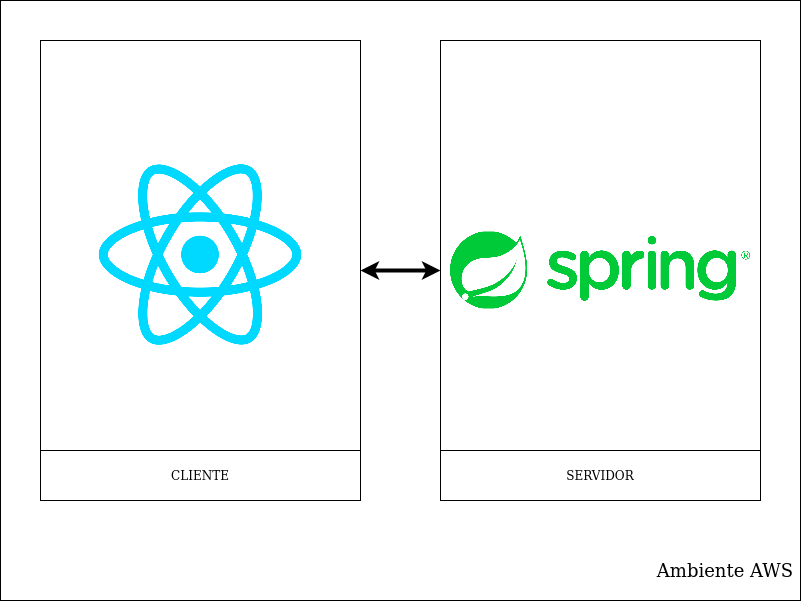
\includegraphics[scale=0.4]{lixt}
  \caption{Arquitetura Lixt}
  \label{fig:cli-srv}
\end{figure}

A comunicação entre estes serviços será feita com o uso do protocolo
\label{sig:https}\hyperlink{s:http}{HTTPS}, que permite a aplicação
cliente realizar chamadas ao servidor através de urls, seja para
buscar informações para apresentar ao usuário ou postar informações
coletadas dele. O framework Spring, além de abstrair a implementação
da lógica de um servidor, implementa \emph{listeners} para estas urls,
auxiliando a criação de pontos na aplicação do servidor focados na
comunicação com a aplicação cliente.

O uso do protocolo HTTPS oferece alguamas vantagens a aplicação
\emph{front-end}, que não precisa esperar uma solicitação ao
\emph{back-end} ser finalizada antes de realizar outras solicitações,
aumentando a repsonsividade da aplicação cliente. Para além disso,
quando combinada ao modelo \label{sig:rest}\hyperlink{s:rest}{REST} na
construção da \label{sig:API} \hyperlink{s:API}{API}, o protocolo HTTP
oferece meios eficientes para que as aplicações se comuniquem.

Como plataforma de servidor, o serviço AWS será utilizado, uma vez que
é oferecida de maneira gratuita para a realização deste projeto, e nele
serão armazenadas algumas instâncias da aplicação \emph{back-end}.
Esta redundância é necessária como forma de garantir a estabilidade do
sistema, de forma que sempre haja alguma disponível para o
processamento de novas requisições, e, em caso de falha numa delas, o
serviço não seja interrompido aos usuários.


\section{Escopo do Projeto}

Lixt é um aplicativo para gerenciamento de listas de compras compartilhadas ou não.

O aplicativo vai seguir a dinâmica de uso abaixo:
\begin{enumerate}
	\item O usuário cria uma lista de compras e insere todos os itens antes da compra;
	\item O usuário inicia um carrinho de compras quando chega ao mercado, nesse momento ele tem a opção de importar para aquele carrinho os itens das listas que ele possui em aberto (que ainda não foram finalizadas), marcando quais listas ele deseja que sejam incluídas. Com o carrinho de compras ele poderá anotar os preços dos itens, riscá-los e ver o total gasto. Ao finalizar a compra as listas são atualizadas, e já aparecem riscados os itens que já foram comprados;
	\item Quando o usuário definir que uma lista não é mais relevante ele poderá deletar a lista ou desmarcar todos os itens, para reutilizar a lista.
\end{enumerate}

A seguir listamos as principais funcionalidades como uma lista de tópicos para facilitar a visualização de quais funcionalidades dependem de outras de forma hierárquica:

\begin{itemize}
	\item \textit{Login}:
		\begin{itemize}
			\item Criar conta;
			\item Redefinir senha;
		\end{itemize}
	\item Editar uma lista:
		\begin{itemize}
			\item Adicionar item:
				\begin{itemize}
					\item Definir nome;
					\item Definir quantidade;
					\item Definir unidade de medida (un. ml, L etc.);
					\item Definir medida;
					\item Adicionar uma categoria:
						\begin{itemize}
							\item Criar nova categoria;
						\end{itemize}
					\item Adicionar um comentário;
					\item Atribuir a um usuário (caso a lista tenha sido compartilhada e pelo menos um convite já tenha sido aceito);
				\end{itemize}
			\item Remover itens;
			\item Convidar pessoas para a lista (apenas quem criou a lista):
				\begin{itemize}
					\item Enviar convite:
						\begin{itemize}
							\item Acompanhar \textit{status} (aceito ou pendente);
							\item Remover convite;
						\end{itemize}
				\end{itemize}
			\item Deletar uma lista;
			\item Limpar uma lista;
		\end{itemize}
	\item Iniciar um carrinho de compras:
		\begin{itemize}
			\item Selecionar listas para compor o carrinho;
			\item Informar o mercado onde a compra será realizada (automaticamente através da localização, se não estiver habilitada será solicitado que o usuário insira o nome do mercado);
			\item Exibir o valor total do carrinho;
			\item Informar a quantidade que será efetivamente comprada naquele momento (o usuário pode ter planejado 10 unidades e apenas comprar 5 naquele momento);
			\item Riscar itens;
			\item Finalizar um carrinho de compras;
		\end{itemize}
	\item Ver estatísticas:
		\begin{itemize}
			\item Selecionar uma lista e ver o total gasto naquela lista ao longo do tempo em um gráfico de linha:
				\begin{itemize}
					\item Selecionar um dos pontos do gráfico e ver detalhes daquela lista;
				\end{itemize}
			\item Selecionar uma lista para ver um gráfico de pizza com os valores médios gastos por categorias naquela lista;
			\item Verificar histórico de preços de um item (tabela com nome do produto, quantidade, marca, preço, mercado e data da compra):
				\begin{itemize}
					\item Selecionar uma lista, dentro da lista selecionada selecionar o produto para ver o histórico;
				\end{itemize}
		\end{itemize}
\end{itemize}

Para o \textit{Minimum Viable Product} (\label{sig:mvp}\hyperlink{s:mvp}{MVP}) vamos implementar as seguintes funcionalidades, as demais ficarão para o próximo semestre:

\begin{itemize}
	\item \textit{Login}:
		\begin{itemize}
			\item Criar conta;
			\item Redefinir senha;
		\end{itemize}
	\item Criar lista de compra:
		\begin{itemize}
			\item Atribuir um nome;
			\item Atribuir uma descrição;
			\item Importar uma lista anterior;
		\end{itemize}
	\item Editar uma lista:
		\begin{itemize}
			\item Adicionar item:
				\begin{itemize}
					\item Definir nome;
					\item Definir quantidade;
					\item Definir unidade de medida (un., ml., L etc);
					\item Definir medida;
					\item Adicionar a uma categoria:
						\begin{itemize}
							\item Criar uma nova categoria;
						\end{itemize}
					\item Adicionar um comentário;
					\item Atribuir a um usuário (caso a lista tenha sido compartilhada e pelo menos um convite já tenha sido aceito);
				\end{itemize}
			\item Remover itens;
			\item Convidar pessoas para a lista (apenas quem criou a lista):
				\begin{itemize}
					\item Enviar convite:
						\begin{itemize}
							\item Acompanhar  status (aceito ou pendente);
							\item Remover convite;
						\end{itemize}
				\end{itemize}
			\item Deletar uma lista;
			\item Limpar uma lista;
		\end{itemize}
	\item Iniciar um carrinho de compras:
		\begin{itemize}
			\item Selecionar listas para compor o carrinho;
			\item Informar o mercado onde a compra será realizada (será solicitado que o usuário insira o nome do mercado manualmente);
			\item Exibir o valor total do carrinho;
			\item Informar a quantidade que será efetivamente comprada naquele momento (o usuário pode ter planejado 10 unidades e apenas comprar 5 naquele momento);
			\item Riscar itens;
			\item Finalizar o carrinho de compras.
		\end{itemize}
\end{itemize}

\subsubsection{Requisitos Funcionais}

Os requisitos funcionais dizem respeito às funcionalidade que o sistema deve ter. A Tabela \ref{reqFuncionais} lista os requisitos funcionais, suas dependências, a sigla e a prioridade de implementação.

\begin{table}[H]
\caption{Requisitos funcionais}
\begin{tabular}{|l|l|l|l|l}
\cline{1-4}
\textbf{Sigla} & \textbf{Descrição}                                                                                                                                                                                                                                               & \textbf{Prioridade} & \textbf{Dependências} &  \\ \cline{1-4}
RF01           & \begin{tabular}[c]{@{}l@{}}\textit{Login}: o usuário deve ser capaz de criar \\ sua conta no aplicativo, definir sua senha e \\ realizar o \textit{login} no sistema.\end{tabular}                                                                                                 & Alta                &                       &  \\ \cline{1-4}
RF02           & \begin{tabular}[c]{@{}l@{}}O sistema deve possibilitar que o usuário \\ crie suas listas de compras e possa atribuir um\\ nome, uma descrição e ter a opção de importar \\ uma lista existente.\end{tabular}                                                     & Alta                & RF01                  &  \\ \cline{1-4}
RF03           & \begin{tabular}[c]{@{}l@{}}Editar uma lista: Possibilita ao usuário o \\ gerenciamento dos itens da lista, como adicionar \\ itens, remover e enviar convites para a lista.\end{tabular}                                                                         & Alta                & RF02                  &  \\ \cline{1-4}
RF04           & \begin{tabular}[c]{@{}l@{}}Iniciar um carrinho de compras: permitir que o \\ usuário importe várias listas de compras, informe \\ o local da compra, o total gasto, quantidade de \\ itens a ser comprados, riscar itens e finalizar \\ o carrinho.\end{tabular} & Alta                & RF03                  &  \\ \cline{1-4}
RF05           & \begin{tabular}[c]{@{}l@{}}Ver estatísticas: ver o histórico de valores \\ pagos em uma lista ao longo do tempo, ver \\ os valores gastos por categorias em uma lista, \\ ver o histórico de preços de um determinado \\ item ao longo do tempo.\end{tabular}    & Média               & RF04                  &  \\ \cline{1-4}
\end{tabular}
\fonte{Os Autores}
\label{reqFuncionais}
\end{table}


\subsubsection{Requisitos Não Funcionais}

De maneira simplificada, os requisitos não funcionais não estão relacionados diretamente às funcionalidades do sistema, mas ao seu funcionamento de um modo geral, ou seja, como ele as funcionalidade serão executadas.

Na Tabela \ref{reqNaoFuncionais} estão elencados os requisitos não funcionais, cada um com sua nomenclatura, categoria e descrição.

\begin{table}[H]
\caption{Requisitos Não funcionais}
\begin{tabular}{llll}
\cline{1-3}
\multicolumn{1}{|l|}{\textbf{Nomenclatura}} & \multicolumn{1}{l|}{\textbf{Descrição}}                                                                                                                                                                                                            & \multicolumn{1}{l|}{\textbf{Categoria}} &  \\ \cline{1-3}
\multicolumn{1}{|l|}{RNF01}                 & \multicolumn{1}{l|}{\begin{tabular}[c]{@{}l@{}}Criptografia das senhas: Por uma questão \\ de segurança as senhas não serão \\ armazenadas diretamente no banco, serão \\ criptografadas antes de serem armazenadas \\ como um \textit{hash}.\end{tabular}} & \multicolumn{1}{l|}{Segurança}          &  \\ \cline{1-3}
\multicolumn{1}{|l|}{RNF02}                 & \multicolumn{1}{l|}{\begin{tabular}[c]{@{}l@{}}Comunicação: A comunicação entre as \\ camadas da aplicação deverá ser feita utilizando \\ o protocolo HTTPS, para garantir a segurança \\ no envio dos dados através da rede.\end{tabular}}        & \multicolumn{1}{l|}{Segurança}          &  \\ \cline{1-3}
\multicolumn{1}{|l|}{RNF03}                 & \multicolumn{1}{l|}{\begin{tabular}[c]{@{}l@{}}Responsividade: O sistema deve exibir \\ corretamente os elementos da interface gráfica \\ nos mais variados tamanhos de celulares.\end{tabular}}                                                   & \multicolumn{1}{l|}{Usabilidade}        &  \\ \cline{1-3}
\multicolumn{1}{|l|}{RNF04}                 & \multicolumn{1}{l|}{\begin{tabular}[c]{@{}l@{}}Internacionalização: O sistema deverá suportar \\ dois idiomas (inglês e português) e suportar \\ que futuramente seja possível adicionar outros \\ idiomas.\end{tabular}}                          & \multicolumn{1}{l|}{Usabilidade}        &  \\ \cline{1-3}
\multicolumn{1}{|l|}{RNF05}                 & \multicolumn{1}{l|}{\begin{tabular}[c]{@{}l@{}}Escalabilidade: O sistema deverá ser projetado \\ para garantir que futuras melhoras e expansões \\ sejam possíveis.\end{tabular}}                                                                  & \multicolumn{1}{l|}{Desempenho}         &  \\ \cline{1-3}
\multicolumn{1}{|l|}{RNF06}                 & \multicolumn{1}{l|}{\begin{tabular}[c]{@{}l@{}}Disponibilidade: O sistema deverá estar disponível \\ aos usuários ininterruptamente\end{tabular}}                                                                                                  & \multicolumn{1}{l|}{Disponibilidade}    &  \\ \cline{1-3}
                                            &                                                                                                                                                                                                                                                    &                                         & 
\end{tabular}
\label{reqNaoFuncionais}
\fonte{Os Autores}
\end{table}

\section{Tecnologias Utilizadas}

As tecnologias que decidimos utilizar foram escolhidas a partir do conhecimento prévio da equipe, da curva de aprendizado e levando em consideração também o tamanho das comunidades que já a utilizam, visando um maior apoio e material de pesquisa.
Dito isso, escolhemos as seguintes tecnologias:

\subsection{Linguagens}

\subsubsection{Back-end}

Decidimos que a linguagem para o \gls{backend} seria o Java. A linguagem se adequa à nossa proposta e atende o paradigma de linguagem orientada a objetos do qual nos foi orientado a utilizar. 
A comunidade de Java é extensa e ativa, contribuindo com muitos materiais e recursos. Ainda podemos destacar que a utilização da linguagem previamente pelos integrantes da equipe também foi impactante na consolidação dessa decisão.

\subsubsection{Mobile}
Para o desenvolvimento da plataforma mobile decidimos utilizar o Javascript. A linguagem possui também uma comunidade ativa e uma variedade de materiais disponíveis e atualizados. Apesar de nem todos os integrantes terem tido contato prévio, por conta da facilidade de assimilação e necessidade de poucos recursos para a configuração do ambiente de desenvolvimento, optamos pelo Javascript.

\subsection{Frameworks e ORMs}

\subsubsection{Back-end}

Para o \gls{backend} decidimos utilizar o \gls{framework} Spring, usando a ferramenta Spring Boot que proporciona agilidade na criação das aplicações pois segue a filosofia de Convention over Configuration\cite{Devopedia2020}, nos poupando de depreender muito tempo nas configurações. Não obstante, a \gls{framework} facilita o desenvolvimento pois nos propicia a utilização de módulos que julgarmos necessários (como Spring MVC e Spring Data JDBC). Além disso, há uma gama vasta de materiais para consultarmos.
Como ferramenta \label{sig:ORM}\hyperlink{s:ORM}{ORM} decidimos usar o Hibernate pela consolidação dele no mercado e o uso amplo em aplicações Java que necessitam de mapeamento relacional dos dados. Por conta da quantidade de modelos da aplicação, julgamos necessário utilizar uma ferramenta que facilitasse esse processo. 

\subsubsection{Mobile}
Na aplicação mobile decidimos utilizar o \gls{framework} React-Native. Esta \gls{framework} gera aplicativos nativos, não necessita de muitos recursos e configurações para montar o ambiente de desenvolvimento e possibilita um conforto maior no desenvolvimento do código por ser uma \gls{framework} Javascript. Não obstante, também é uma \gls{framework} com larga quantidade de recursos para consulta além de uma comunidade muito ativa.

\subsection{Banco de dados}
O banco de dados que escolhemos foi o MySQL pois precisávamos para a nossa proposta de um banco de dados relacional e que fosse possível de ser hospedado na AWS. Verificamos que o MySQL cobria não apenas esses critérios mas também possui uma ferramenta gráfica (MySQL Workbench) que facilita a visualização e a operação do banco. Além disso os integrantes da equipe já tiveram experiências com a ferramenta anteriormente.

\subsection{Gerenciamento de tarefas}
Para o gerenciamento das tarefas optamos pela ferramenta Trello por ser gratuita, de fácil manuseio e visualização.
Além disso, o Trello figura entre as ferramentas que foram utilizadas com sucesso nos semestres anteriores durante o desenvolvimento de projetos.

\subsection{Versionamento}
Para o controle de versão do desenvolvimento da aplicação optamos pelo Git com repositório no Github. Esta escolha foi realizada devido à experiência prévia da equipe com a ferramenta e pela quantidade de recursos oferecidos pela plataforma na gestão do desenvolvimento de aplicações.
Para o versionamento do projeto utilizamos o Apache Subversion (SVN). Concentramos no repositório fornecido pelos professores todas as entregas previstas (incluindo as versões atualizadas dos códigos do repositório externo do Github).



%%% Local Variables:
%%% mode: latex
%%% TeX-master: "../proposta"
%%% End:


\section{Escalabilidade}

A escalabilidade da aplicação é sua capacidade de se adequar a um
amplo volume de requisições, mantendo a estabilidade do sistema e a
velocidade de respostas. Um sistema escalável está apto para responder
adequadamente nestes momentos, assim como liberar seus recursos em
momentos com poucas requisições.

Por se tratar de algo relativo ao processamento de requisições, a
escalabilidade diz respeito ao \gls{backend}, que centraliza os
pedidos dos usúarios. A camada cliente por outro lado, por focar
exclusivamente na lógica de visualização, e rodar em dispositivos
mobile, não exige tanta capacidade de processamento, e a
escalabilidade não é uma preocupação para esta camada.

Como foi mencionado, a aplicação \gls{backend} ficará armazenada na
plataforma Amazon AWS. Existe um processo da ferramenta de integração
contínua Jenkins para aumentar o número de instâncias ativas em
produção, e este processo será acionado em momentos com intenso volume
de requisições.


%%% Local Variables:
%%% mode: latex
%%% TeX-master: "../../desenho"
%%% End:


\section{Mantenibilidade da aplicação}

É fundamental para o desenvolvimento do projeto, tanto o previsto
quanto em avanços posteriores, que a aplicação atinja um nível adequado
de qualidade, e para tanto certos requisitos de manutenibilidade devem
ser estabelecidos.  Estes requisitos permitem a

\subsection{\emph{Logs}}

Como forma de monitorar a aplicação em tempo de execução,
especialmente na camada de servidor, \emph{logs} serão usados para
registrar o estado dos objetos. A ferramenta Log4j será usada, uma vez
que os membros do time já tem mais familiaridade com ela. Esta
ferramenta perimite o registro em diversos níveis, como
\begin{itemize}
  \em
\item info
\item debug
\item warn
\item error
\end{itemize}
e pode ser configurada para que apenas os dois últimos
sejam registrados no ambiente de produção. Desta forma a cada ponto de
falha da aplicação um log de nível apropriado será colocado para que
problemas sejam rapidamente identificados, analisados e resolvidos.

\subsection{Integração Contínua}

Visando manter o serviço sempre atualizado para o usuário, a
ferramenta de integração contínua Jenkins foi selecionada para a
implantação da aplicação \emph{back-end} em produção. Ela
permite, a partir do código no repositório git, a execução de testes,
o build e o \emph{deploy} para o ambiente de produção, automatizando tarefas
complicadas de se executar em máquinas remotas.

%% front-end ......

\subsection{\emph{Code Conventions}}

As convenções de código são acordos internos ao time que visam
estandartizar a forma como os diversos integrantes do time produzem
seus códigos.  Elas visam facilitar o entendimento mútuo entre os
integrantes do time, de modo o estilo de progamação seja indistiguível
e independente de seus autores.  Geralmente, as convenções de código
estabelecem estilos para se organizar o código textualmente, isto é,
dizem respeito a forma como nomes de variáveis são escolhidas e
comentários são posicionados, por exemplo.

As convenções adotadas são baseadas na especificação da
\citeauthor{Oracle1997}, de 1997. Esta é comumente usadas para o
desenvolvimento na linguagem Java, e muito próxima do padão adotado em
JavaScript, e vale destacar o seguintes pontos:
\begin{itemize}
\item Minimizar o uso de variáveis, funções e objetos globais.
\item As declarações globais estarão preferencialmente no início do arquivo.
\item Declarar as variáveis próximo do ponto onde elas serão inicializadas.
\item A indentação é de 4 espaços.
\item Linhas mais longas que 80 caracteres serão quebradas e
  indentadas a 8 espaços.
\item Pacotes e variáveis com nomes curtos, em \texttt{camelCase} e substantivos.
\item Classes e interfaces em \texttt{CamelCase} e substantivos.
\item Métodos em \texttt{camelCase} e verbos.
\item Constantes em \texttt{UPPER\_CASE}.
\end{itemize}

No entanto, especificamente para a linguagem Java,
\begin{itemize}
\item Classes e métodos devem ser documentados com um comentário na
  seguinte forma, uma vez que as IDEs reconhecem este formato e
  formatam o text na forma de \emph{pop-ups} quando o cursor está
  sobre uma referência a esta classe.
\begin{verbatim}
/**
 * Class ListService
 *
 * Implementar endpoints para as funcionalidades de lista.
 */
\end{verbatim}
\end{itemize}
%%% Local Variables:
%%% mode: latex
%%% TeX-master: "../../desenho"
%%% End:


\include{section/segurança}

\section{Viabilidade Financeira}

O projeto de análise de viabilidade financeira consiste em averiguar a garantia de lucro sobre as despesas do projeto. Portanto, nesse projeto será descrito cada processo a fim de fazer essa verificação.

\subsection{Gerenciamento de Custos}

Nesse tópico, serão abordados temas de investimento inicial e de desenvolvimento do projeto, incluindo tópicos de análise de requisitos, desenvolvimento, manutenções e imprevistos.

\subsubsection{Análise de Requisitos e Desenvolvimento}

Para iniciar o projeto, é necessário fazer os primeiros planejamentos, elicitação de requisitos, abstrair e concretizar as primeiras ideias e fazer os primeiros planejamentos (diagramas, cronogramas e documentação). Logo após, o projeto chega na fase de desenvolvimento, onde é começado a se tornar real.

Contudo, o projeto não vai possuir nenhum custo de análise e implementação do sistema, devido ao fato de ser um projeto educacional.

\subsubsection{Manutenções}

Inevitavelmente, manutenções do sistema ocorrerão pós finalização do projeto e estar devidamente funcional em produção. Contudo, os custos de manutenções também não serão cobrados, devido a ser um projeto educacional.

\subsection{Custos de deploy e de Ambiente de Produção}

Nesse tópico, são apresentados os custos de manter o sistema funcional e disponível para os usuários. Desse modo, será feito uma previsão anual de cada plataforma utilizada:

\subsubsection{Frontend} 

Tendo em vista que o projeto é \textit{mobile} voltado para dispositivos Android, será publicado na PlayStore, estimando um valor de 25.00 USD anual. 

\subsubsection{Backend}

Inicialmente gratuíto no Amazon EC2, sendo permitido 750h de instâncias por mês durante o período de 12 meses.

A partir do momento que for necessário grande porte, será indicado o plano Sob Demanda do Amazon EC2, que garante viabilidade econômica e estratégica (visto que o preço é calculado a partir do uso). 

Nesse plano, o custo de transferência de dados (ou seja, entrada e saída de dados) geram o valor de, na região de São Paulo, no máximo 0,15 USD por GB.

Na \autoref{fig:prices-ec2}, seguem os preços dos planos Sob Demanda na região de São Paulo para Linux usando tipo de instância geral com 1 vCPU.

\begin{figure}[h]
  \centering
  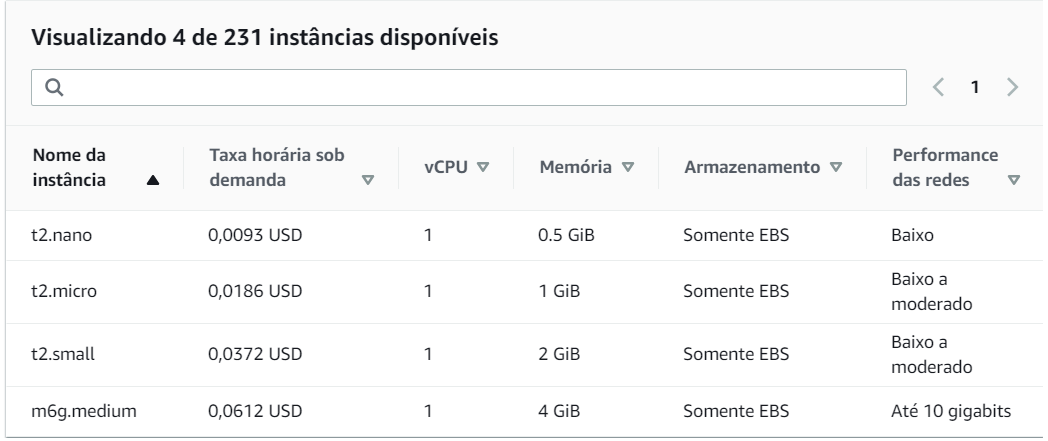
\includegraphics[scale=0.6]{prices-ec2}
  \caption{Preços do Amazon EC2 - Sob Demanda \\ \cite{AmazonEC2}}
  \label{fig:prices-ec2}
\end{figure}

\subsubsection{Banco de Dados} 

Inicialmente gratuíto no Amazon RDS, sendo permitido 750h de instâncias durante o período de 12 meses. O Amazon RDS possui suporte a vários Sistemas Gerenciadores de Banco de Dados (SGBD), incluindo o MySQL, que foi o SBGD optado para desenvolver a aplicação Lixt.

A partir do momento que for necessário grande porte, será indicado o plano Sob Demanda do Amazon RDS, que garante viabilidade econômica e estratégica (visto que o preço é calculado a partir do uso).

Na \autoref{fig:prices-rds}, seguem os preços dos planos Sob Demanda na região do Leste dos EUA (única opção disponível em 07/06/2021).

\begin{figure}[h]
  \centering
  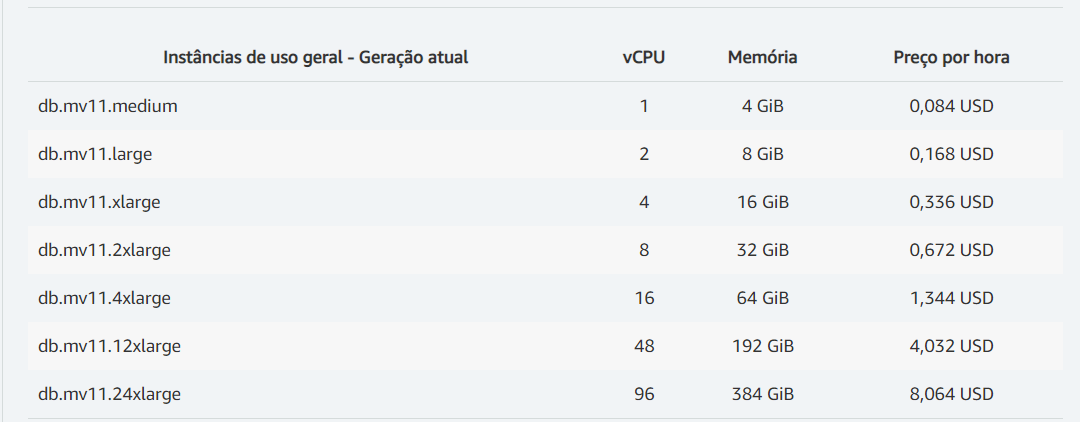
\includegraphics[scale=0.6]{prices-rds}
  \caption{Preços do Amazon RDS - Sob Demanda \\ \cite{AmazonRDS}}
  \label{fig:prices-rds}
\end{figure}	

\subsection{Medidas de Obtenção de Retorno Financeiro}

Para gerar uma receita positiva a fim de obter lucro, haverá duas formas principais de retorno financeiro:
\begin{itemize}
	\item \underline{Cobrança do aplicativo}: O aplicativo estará disponível gratuitamente na PlayStore, não gerando, portanto, retorno financeiro.
	\item \underline{Propaganda/Recomendação}: Será utilizado mediador de anuncio AdMob (responsável por conectar aplicações e anunciantes), onde o valor varia por visualizações de anúncios e cliques neles. Contudo, no próprio site do admob, é citado um caso no qual houve 300.000 downloads e recebia, através do AdMob, 100 USD por dia. \cite{GoogleAdMob}
\end{itemize}
s

% ------------------------------------------------------------------------------
% ------------------------------------------------------------------------------
% Coloquem aqui o include dos capitulos de voces
% e o arquivo correspondente na pasta capitulos
\chapter{Tecnologias Utilizadas}

As tecnologias que decidimos utilizar foram escolhidas a partir do conhecimento prévio da equipe, da curva de aprendizado e levando em consideração também o tamanho das comunidades que já a utilizam, visando um maior apoio e material de pesquisa.
Dito isso, escolhemos as seguintes tecnologias:

\section{Linguagens}

\subsection{Back-end}

Decidimos que a linguagem para o back-end seria o Java. A linguagem se adequa à nossa proposta e atende o paradigma de linguagem orientada a objetos do qual nos foi orientado a utilizar. 
A comunidade de Java é extensa e ativa, contribuindo com muitos materiais e recursos e além disso podemos destacar que a utilização da linguagem previamente pelos integrantes da equipe também foi impactante na consolidação dessa decisão.

\subsection{Mobile}
Para o desenvolvimento da plataforma mobile decidimos utilizar o Javascript. A linguagem possui também uma comunidade ativa e uma variedade de materiais disponíveis e atualizados. Apesar de nem todos os integrantes terem tido contato prévio, por conta da facilidade de assimilação e necessidade de poucos recursos para a configuração do ambiente de desenvolvimento, optamos pelo Javascript.

\section{Frameworks e ORMs}

\subsection{Back-end}

Para o back-end decidimos utilizar o framework Spring, usando a ferramenta Spring Boot que proporciona agilidade na criação das aplicações pois segue a filosofia de Convention over Configuration\cite{Devopedia2020}, nos poupando de depreender muito tempo nas configurações. Não obstante, a framework facilita o desenvolvimento pois nos propicia a utilização de diversos módulos que julgarmos necessários. Como Spring MVC e Spring Data JDBC. Além disso, há uma gama vasta de materiais para consultarmos.
Como ferramenta ORM decidimos usar o Hibernate pela consolidação dele no mercado e o uso amplo em aplicações Java que necessitam de mapeamento relacional dos dados. Por conta da quantidade de modelos da aplicação, julgamos necessário utilizar uma ferramenta que facilitasse esse processo. 

\subsection{Mobile}
Na aplicação mobile decidimos utilizar o framework React-Native. Esta framework gera aplicativos nativos, não necessita de muitos recursos e configurações para montar o ambiente de desenvolvimento e possibilita um conforto maior no desenvolvimento do código por ser uma framework Javascript. Não obstante, também é uma framework com larga quantidade de recursos para consulta além de uma comunidade muito ativa.

\section{Banco de dados}
O banco de dados que escolhemos foi o MySQL pois precisávamos para a nossa proposta de um banco de dados relacional e que fosse possível de ser hospedado no Heroku. Verificamos que o MySQL cobria não apenas esses critérios mas também possui uma ferramenta gráfica (MySQL Workbench) que facilita a visualização e a operação do banco e além disso os integrantes da equipe já tiveram experiências com a ferramenta anteriormente.

\section{Gerenciamento de tarefas}
Para o gerenciamento das tarefas optamos pela ferramenta Trello por ser gratuita, de fácil manuseio e visualização.
Além disso, a ferramenta figura entre as ferramentas que foram utilizadas com sucesso nos semestres anteriores em Projetos.



%%% Local Variables:
%%% mode: latex
%%% TeX-master: "../proposta"
%%% End:

% ------------------------------------------------------------------------------
% ------------------------------------------------------------------------------

\phantompart
\postextual

\bibliography{referencias/referencias}

\end{document}
%%% Local Variables:
%%% mode: latex
%%% TeX-master: t
%%% End:
